Modelling refers to the process of creating a simplified representation or
approximation of a real-world system, process, or phenomenon in order to improve
understanding and facilitate analysis. It is commonly used in the fields of
physics and mathematics, where mathematical equations are used to depict reality
and capture the important factors of a particular system in a manageable and
understandable format~\cite{witelski2015methods}.

In the field of optimization, there is an extensive body of literature on the
development of mathematical programming models for a wide range of
problems~\cite{papadimitriou1998combinatorial,nocedal2006numerical,williamson2011design}.
One of the key advantages of this approach is that it
allows for the application of standard solvers that can be used to find
solutions to diverse problems. This can be attributed to the fact that the model
encapsulates all the information required by a generic solver to address any
problem in a principled manner.

In the field of meta-heuristics, to the best of our knowledge, there is no
established concept of a ``model''. Despite this, there is interest within the
community in the development of such models that allow the development of
solvers that tackle problems in a black-box fashion. However, there is also some
skepticism about the feasibility of this. Nonetheless, if we attempt to identify
the characteristics that must be encoded in a model in order for it to be
available to a meta-heuristic solver of this kind, certain key aspects must
certainly be considered, such as:

\begin{itemize}
      \item \textbf{Instance Parameters}: Description of the problem instance.
      \item \textbf{Decision Space}: Description of the solution and component
            structure. Moreover, it should detail concepts such as: empty
            solution, partial solution, complete solution and feasibility.
      \item \textbf{Construction Rules}: Description of how components can be
            joined to form a feasible solution.
      \item \textbf{Objective Function \& Bounds}: Description of how partial or
            complete solutions could be evaluated.
\end{itemize}

Therefore, an approach that incorporates these considerations could facilitate a
principled approach to the problem, allowing for the use of meta-heuristics as
solvers in the same manner as traditional solvers are utilized in mathematical
programming.

\subsection{Frameworks}

In the literature, two noteworthy studies that adopt a practical approach to
modeling in the context of meta-heuristics are those by Vieira et
al.~\cite{vieira2009uma} which proposes a Python framework for experimentally
testing meta-heuristics and the API developed by Outeiro et
al.~\cite{outeiro2021application} which builds upon these concepts and applies
them to CS approaches. The upcoming sections provide a succinct summary of the
most relevant features and contributions of these works.

\begin{figure}[h]
      \centering
      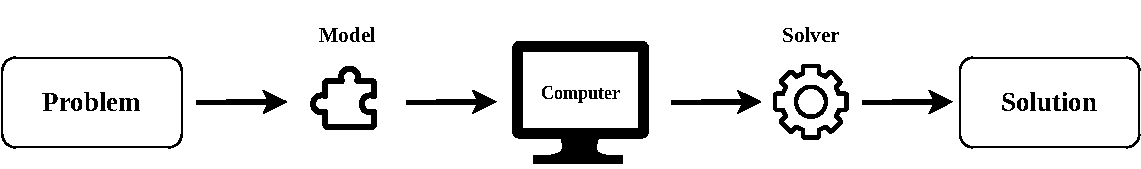
\includegraphics[width=\textwidth,keepaspectratio]{../assets/modelling/modelling.pdf}
      \caption{Principled Modelling Framework}
      \label{fig:problem-solving}
\end{figure}

\subsubsection{Python Optimization Framework (POF)}

This framework, developed in the context of the work by Vieira et
al.~\cite{vieira2009uma}, is the first to implement the modeling principles for
meta-heuristics. It does so by providing an ``external'' and ``internal'' interface.
The external interface is designed for use by meta-heuristic developers who are
interested in the implementation of solvers, while the internal interface is
designed for individuals who want to engage with the framework from a
problem-solving perspective and are not interested in the implementation details
of the algorithms.

Generally, the POF is implemented by  them means of three main classes:
\texttt{Problem}, \texttt{Solver} and \texttt{Simulator}:

\begin{itemize}
      \item \textbf{\texttt{Problem}}: This class is where the modeling-related
            aspects are implemented. Specifically, the solution generation and
            evaluation are described by a series of classes and methods that, when
            implemented, comprise the ``model''. These classes and methods allow the user
            to specify how solutions are generated, how they can be modified to improve
            them, and how they are evaluated, thus constituting the ``internal'' interface.
      \item \textbf{\texttt{Solver}}: This class is where meta-heuristics can be implemented in
            a problem-independent manner. By calling upon the methods defined int the \texttt{Problem}
            class the development of these algorithms is standardized and constitutes the ``external''
            interface of this framework.
      \item \textbf{\texttt{Simulator}}: This class servers as a general-purpose utility
            that allows the step-by-step execution of an implemented \texttt{Solver} with an
            implemented \texttt{Problem}, thus being responsible for the execution of the
            algorithms and gathering of solutions.
\end{itemize}

Furthermore, this work defines several primitives that a model must implement in
order to be as generic as possible and be applied to different situations. These
primitives include the enumeration of moves, such as the addition or removal of
components. These concepts are further refined in the API for constructive
search proposed by Outeiro et al.~\cite{outeiro2021application}.

\subsubsection{Not Another Software Framework for Nature-Inspired Optimisation
      --- Constructive Search}

In his work, Outeiro et al.~\cite{outeiro2021application} builds upon the
concepts presented in the POF and an existing implementation of a framework for
local search~\cite{fonseca2021nasf4nio}, further unifying the concepts and
providing both a conceptual model and an implementation of an API (in the C
Programming Language) for constructive search --- ``nasf4nio-cs''.

Specifically, this API refines the model definition (the \texttt{Problem} class
in the POF) by narrowing down the specifications into a small subset of
operations and data structures. These elements, when combined, allow for the
complete characterization of a model and the implementation of generic
meta-heuristics.

In terms of the data structures, the API defines the following:

\begin{itemize}
      \item \textbf{\texttt{Problem}}: This data structure is responsible for recording
            all the problem instance specific features and other relevant information
            that may be acquired and that pertains to the problem at hand and thus not
            being changed by the solver in any way
      \item \textbf{\texttt{Solution}}: This data structure is responsible for storing the
            data pertaining to a complete/partial solution for a particular problem
            instance.
      \item \textbf{\texttt{Component}}: This data structure stores the data relative to a
            component from the ground set $\mathcal{G}$ that may added, removed, permitted
            or forbidden w.r.t. a given solution.
\end{itemize}

With regards to the operations, by focusing on the ones that are specifically
utilized for manipulating solutions and disregarding those used for
implementation details such as inspection, assignment and memory management, we can
categorize them into three primary groups.

\begin{itemize}
      \item \textbf{Generation}: In this category we find operations such
            as:~\textit{emptySolution} and~\textit{heuristicSolution}~which are used to
            generate solutions for a given problem.
      \item \textbf{Construction}: Under this category fall operation that
            allow a partial solution to be further improved constructively. These include
            the functions \textit{applyMove}, \textit{enumMove}, \textit{heuristicMove},
            \textit{heuristicMoveWOR}, \textit{randomMove} and \textit{randomMoveWOR},
            which allow for the application, enumeration and selection of moves.
            In this context, a move refers to the modification of a given solution by
            performing an action on its components.
      \item \textbf{Evaluation}: In this category appear functions such
            as \textit{getObjectiveVector} and \textit{getObjectiveLB} which allow for
            evaluation of the quality of the solution w.r.t. objective value and bounds.
\end{itemize}

In summary, this API is a comprehensive tool for modeling meta-heuristics in a
principled manner. Although it is not fully developed to support local search
approaches, it is in a state where it can be easily used and adapted, making it
an essential component of our work. The current specification allows
for the implementation of meta-heuristic solvers in a problem-independent
fashion, adhering to the philosophy proposed by Vieira et
al.~\cite{vieira2009uma}, thus allowing for experimentally assessing the pros
and cons of meta-heuristic approaches.